% IEEE COINS 2026 Conference Paper - Double-Blind Submission
% Track 3: AI Architectures and Systems Design
\documentclass[conference]{IEEEtran}

\usepackage[utf8]{inputenc}
\usepackage[T1]{fontenc}
\usepackage{amsmath,amssymb}
\usepackage{graphicx}
\usepackage{booktabs}
\usepackage{multirow}
\usepackage{url}
\usepackage{hyperref}
\usepackage{xcolor}
\usepackage{balance}
\usepackage{cite}
\usepackage{siunitx}
\usepackage{dblfloatfix}

% Double-blind: no author-identifying info
\hypersetup{hidelinks}

% TODO marker for values pending hardware measurement
\newcommand{\TODO}[1]{\textcolor{red}{\textbf{[TODO: #1]}}}

% --- STM32 latency (DWT cycle counter, 10 timed runs, 32x32 native LCE) ---
\newcommand{\STMLATAVG}{50.29\,ms}
\newcommand{\STMLATMIN}{50.29\,ms}
\newcommand{\STMLATMAX}{50.30\,ms}
\newcommand{\STMARENAKIB}{110\,KiB}

\begin{document}

\title{Binarized Wake-Up of Conversational Agents on an Industry-Grade High-Performance Microcontroller}

% Double-blind: authors hidden
\author{
\IEEEauthorblockN{Paper ID: 2836}
\IEEEauthorblockA{(Double-Blind Review --- Authors Omitted)}
}

\maketitle

% ============================================================
\begin{abstract}
Quantization is an effective technique for field-deployment of neural networks (NNs) within applications on resource-limited devices.
A representative case is the wake-up of conversational agents, where a camera-bearing edge node continuously monitors the environment to detect the visual trigger through which a user starts the interaction with the agent.
While the state of the art on the WakeVision person-detection benchmark spans floating-point and up to 4-bit quantized models, binary quantization has not been addressed in the literature yet.
Binarization frequently allows the implementation of high resource-efficiency solutions; however, it is challenging to implement since, differently from the other quantization types, it requires specific binary operations, that are not provided by standard off-the-shelf machine learning libraries for microcontrollers.
To explore the issue, we study two binary deployments on a STM32H7B3I-DK high-end microcontroller.
First, we use NAS-BNN, a framework dedicated to optimizing binary NNs, to discover and deploy a binary convolutional NN via the Larq Compute Engine; to fit the memory budget, we resort to a 16-tile spatial input-streaming scheme.
Second, we binarize the official Wakevision 4-bit Samy model using the CBin-NN inference engine, achieving the best overall trade-off in terms of latency, memory footprint, and energy consumption. This highlights the effectiveness of tightly coupling hardware-aware model design with deployment via a dedicated, binary-optimized runtime. These findings set the reference for minimal footprint deployment of NN solutions for the visual wake-up of conversational agents and indicate promising directions for future research.
\end{abstract}

\begin{IEEEkeywords}
Binary Neural Networks, CBin-NN, Conversational Agents, Larq Compute Engine, MCU deployment, Microcontrollers, Neural Architecture Search, TinyML,  Visual Wake-Up, WakeVision
\end{IEEEkeywords}

% ============================================================
\section{Introduction}
\label{sec:intro}

The wake-up of conversational agents is a typical TinyML application, in which a camera-bearing edge device continuously monitors its environment to detect the visual trigger through which a user can initiate interaction with the agent.
This always-on workload demands neural network inference under kilobyte-scale RAM and milliwatt power budgets~\cite{banbury2021micronets}, motivating aggressive quantization.

WakeVision~\cite{banbury2025wakevision} has recently emerged as a benchmark for visual wake-up tasks on resource-constrained devices, targeting the detection of person-presence events that can activate downstream interactive systems.
Unlike generic image-classification benchmarks, WakeVision focuses on always-on, low-power visual sensing and therefore captures the accuracy-efficiency trade-offs that are central to TinyML deployments.
While the state of the art on WakeVision spans floating-point and up to 4-bit integer quantization, extreme binary quantization, restricting both weights and activations to $\{-1,+1\}$ has not been addressed for this task yet.

Binary Neural Networks (BNNs) replace floating-point multiply-accumulate with single-cycle XNOR and popcount instructions, yielding up to $32\times$ model compression and throughput gains on hardware with native binary support~\cite{rastegari2016xnor, sze2017efficient, dabbous2025binary}, but they are challenging to deploy because, unlike higher bit quantization schemes, they require specific binary operations, that are not included in popular machine learning libraries for microcontroller units (MCUs).

Neural Architecture Search (NAS) complements quantization by automating the design of models that lie on the Pareto front of accuracy versus computational cost~\cite{baymurzina2022review, liberis2021munas}. Hardware-aware methods such as MCUNet~\cite{lin2020mcunet} integrate memory and latency constraints directly into the search, so that the resulting architectures fit a target device by construction.

The NAS-BNN framework~\cite{lin2025nasbnn} applies NAS to the binary domain, using evolutionary search over a weight-sharing supernet to find efficient binary architectures on ImageNet~\cite{deng2009imagenet} and MS~COCO~\cite{lin2014microsoft}.
However, NAS-BNN reports no Flash footprints, activation memory sizes, nor inference latency on physical hardware.
Deployment of NAS-discovered binary models on MCUs and performance comparison with alternatives remains largely unexplored.

This paper addresses this gap by quantitatively comparing the binary deployment workflow supported by NAS-BNN with the binarization of a state of the art quantized model using an optimized engine such as CBin-NN~\cite{sakr2024cbinnn}.
To accomplish this, we first build a complete pipeline from NAS-BNN architecture search through Larq Compute Engine (LCE)~\cite{bannink2021larq} export to TensorFlow Lite Micro (TFLM)~\cite{david2021tflitemicro} execution on an STM32H7B3I-DK (Cortex-M7, 280\,MHz, 1.4\,MB SRAM), reporting the first measured latency, RAM, and Flash figures for NAS-discovered binary models on a Cortex-M device.
This process reveals a fundamental constraint not visible from operation counts: at full $128\times128$ resolution, the activation occupancy of NAS-BNN models exceed the STM32H7B3I-DK's available SRAM, driven by float32 skip-connection tensors that span multiple binary stages and accumulate to hundreds of kilobytes.
NAS-BNN also lacks a binary-runtime-compatible export path: the framework searches a binary weight space but produces standard PyTorch models with no notion of a target binary inference backend, so without an explicit conversion step the binary weights would be executed as float operations rather than XNOR-popcount, negating the efficiency argument entirely.

On the other hand, a tailored architecture (Key 4 in \cite{pighetti2024exploring}), exploiting a 16-tile spatial input-streaming optimization, keeps full-resolution inference within the 480 KiB SRAM budget at 80.41\% accuracy and 800 ms.
This raises a key question: can a model designed from scratch under MCU constraints outperform a NAS-discovered model that is subsequently adapted to meet those hardware requirements?
To answer this, we binarize the official Wakevision 4-bit Samy model and convert it to C using the CBin-NN inference engine~\cite{sakr2024cbinnn}.
Our analysis shows that this CBin-NN-deployed binary network achieves the best overall trade-off in latency, memory footprint, power and energy, at acceptable accuracy providing quantitative evidence that hardware-aware model design and a dedicated binary runtime jointly outperform a NAS pipeline that ignores deployment constraints.

The main contributions of this work are as follows.
\begin{enumerate}
    \item We introduce a complete deployment pipeline from NAS-BNN architecture search through LCE TFLite export to Cortex-M7 firmware, including a 16-tile spatial streaming scheme that fits the 480\,KiB SRAM budget.

    \item We conduct the binarization of the Samy model, a state of the art 4-bit WakeVision reference model and its C-language deployment via CBin-NN, achieving the best trade-off across  latency, RAM, Flash, and energy on the target STM32H7B3I-DK MCU.

    \item We provide an empirical comparison of NAS-BNN-derived models, two state of the art WakeVision models, and the binarized counterpart of one of them, evaluated under identical MCU deployment conditions. The results establish a reference point for minimal-footprint visual wake-up systems for conversational agents.
\end{enumerate}

The remainder of the paper is organized as follows.
Section~\ref{sec:related} reviews related work.
Section~\ref{sec:method} presents the methodology.
Section~\ref{sec:results} reports the results, while
Section~\ref{sec:discussion} discusses the findings and Section~\ref{sec:conclusion} concludes the paper.

\begin{figure*}[h]
  \centering
  
\includegraphics[width=0.8\linewidth]{fig_pipeline.pdf}
  \caption{End-to-end NAS-BNN deployment pipeline.}
  \label{fig:pipeline}
\end{figure*}

% ============================================================
\section{Related Work}
\label{sec:related}

\subsection{Binary Neural Networks}

BNNs constrain weights and activations to $\{-1, +1\}$, reducing multiply-accumulate to XNOR-popcount~\cite{rastegari2016xnor} operations.
Bi-RealNet~\cite{liu2018birealnet} improved representational capacity through real-valued skip connections. ReActNet~\cite{liu2020reactnet} introduced generalized activation functions to reduce binarization information loss.
MoBiNet~\cite{phan2020mobinet} applied depthwise separable binary convolutions for mobile use.
BNN pruning methods~\cite{li2020bnnpruning} further compress binary models by removing redundant filters guided by weight-flipping frequency.
Despite these advances, the deployability of BNNs on microcontroller hardware has received limited attention. The specialized LCE \cite{bannink2021larq} and CBin-NN \cite{sakr2024cbinnn} runtimes provide binary-kernel inference, but their integration into a full NAS-to-MCU pipeline has not been demonstrated.

\subsection{NAS for Efficient Models}

NAS automates architecture design by searching over parameterized spaces~\cite{baymurzina2022review}.
Hardware-aware NAS methods such as FBNet~\cite{wu2019fbnet} and $\mu$NAS~\cite{liberis2021munas} incorporate latency or memory constraints directly into the search objective.
MCUNet~\cite{lin2020mcunet} jointly optimizes the neural architecture and inference library for microcontroller deployment, achieving 85.9\% on WakeVision at 56\,M-MACs (4--8-bit) with 410\,ms on a Cortex-M7.
NAS-BNN~\cite{lin2025nasbnn} targets binary search spaces, using a weight-sharing supernet and an evolutionary algorithm to find Pareto-optimal architectures. However, the deployment of the models found by NAS-BNN on physical MCUs is not reported.
A preliminary exploration of NAS for BNNs specifically on the WakeVision benchmark was presented in~\cite{pighetti2024exploring}. The present work extends that line to a complete, measured deployment pipeline on a Cortex-M7 MCU.

\subsection{TinyML Deployment and Person Detection}

TinyML brings neural inference to devices operating under kilobyte-scale memory budgets~\cite{banbury2021micronets, mittal2024comprehensive}.
The MLPerf Tiny benchmark~\cite{banbury2021mlperftiny} standardizes evaluation across tasks including person detection.
WakeVision~\cite{banbury2025wakevision} provides a large-scale, fine-grained benchmark specifically for TinyML person detection, with over six million images and a test set of 55{,}762 balanced samples.
TensorFlow Lite Micro (TFLM)~\cite{david2021tflitemicro} is a widely used embedded inference runtime for microcontroller-class devices and Larq Compute Engine~\cite{bannink2021larq} (LCE) extends it with bit-packed binary convolution kernels that exploit SIMD instructions on Cortex-M and Cortex-A processors. The LCE framework allows for seamless definition, training, evaluation and deployment of BNNs.
% ============================================================
\section{Methodology}
\label{sec:method}

\subsection{NAS-BNN Supernet and Diversity-Aware Pareto Selection}

Our pipeline builds on the NAS-BNN~\cite{lin2025nasbnn}, which provides a searchable family of BNNs rather than a single fixed architecture. In NAS-BNN, candidate architectures are sampled as subnetworks from a shared over-parameterized supernet, allowing binary architectures to be evaluated without training each one independently from scratch.
The supernet is a sequence of binary convolutional blocks, each parameterized by six choices: output channels, kernel size ($3\times3$; $5\times5$; $7\times7$), two grouping factors, a skip-connection flag, and stride.
Computational cost is measured in composite operations:
\begin{equation}
\text{OPs} = \text{FLOPs} + \frac{\text{Int8OPs}}{4} + \frac{\text{BOPs}}{32}
\label{eq:ops}
\end{equation}
where FLOPs refers to floating-point operations in the full-precision stem, Int8OPs to 8-bit operations, and binary operations (BOPs)~\cite{lin2025nasbnn}.
The $1/32$ factor follows the convention used in NAS-BNN, which counts one BOP as one thirty-second of a FLOP to account for the lower hardware cost of bitwise XNOR-popcount computation~\cite{sze2017efficient}.
For Key~4, raw binary operations total $\sim$141\,M-BOPs (the composite 4.40~M-OPs figure normalizes this by dividing by 32).

NAS-BNN explores this search space through evolutionary search.
New candidate architectures are generated by selecting previously evaluated architectures as parents and applying mutation operators to their architectural choices.
In the original NAS-BNN algorithm, parents are sampled exclusively from the current Pareto front, which may lead to premature convergence and reduced architectural diversity.
We introduce a diversity-aware variant of Pareto-based parent selection: a three-tiered probabilistic scheme inspired by NSGA-II~\cite{deb2002nsga2} that draws 70\% of parents from the current Pareto front (exploitation), 20\% from previously visited but non-Pareto architectures (re-exploration), and 10\% at random (diversity).
This preserves genetic diversity without any additional architecture evaluations.

\subsection{NAS-BNN End-to-End Pipeline}

A critical obstacle to deploying NAS-BNN models is that the original supernet relies on dynamic PyTorch~\cite{paszke2019pytorch} modules that cannot be exported directly. Fig.~\ref{fig:pipeline} summarizes our end-to-end NAS-BNN deployment pipeline, which resolves this issue through architecture selection, static model instantiation, fine-tuning, LCE export, and MCU deployment.

After selecting an architecture from the Pareto front, we first instantiate a static model in which all dynamic choices are replaced with fixed convolutional layers. The sign of the batch-normalized weights is pre-computed and the resulting $\{-1,+1\}$ values are baked into the static model, eliminating runtime sign operations and producing a clean export graph.
The static model is then exported to the TensorFlow Lite format using the LCE converter, which replaces standard float convolutions with \texttt{LceBconv2d} and \texttt{LceQuantize} custom operators that pack 32 binary weights per 32-bit word. To verify numerical correctness, we run forward passes on both the PyTorch source model and the TFLite artifact for 1{,}000 identical inputs and check that softmax outputs agree to within 0.05\%.

Finally, the architectures are fine-tuned from the supernet weights on the full WakeVision training set using knowledge distillation~\cite{hinton2015distilling}, with the supernet's largest and smallest sub-networks as teachers, label smoothing ($\epsilon = 0.1$), and cosine annealing for 30 epochs.

\subsection{STM32 Deployment}
\label{subsec:stm32}

\begin{figure}[t]
  \centering
  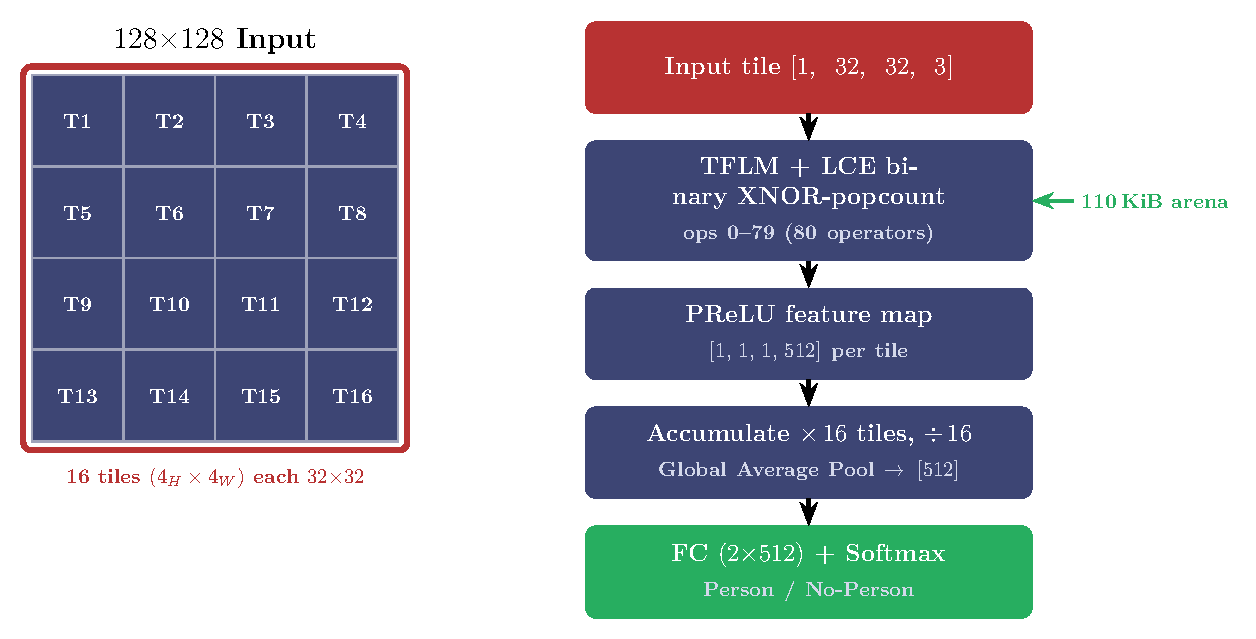
\includegraphics[width=\columnwidth]{fig_tiling.pdf}
  \caption{16-tile 2D spatial streaming ($4_H{\times}4_W$) and per-tile inference flow.}
  \label{fig:tiling}
\end{figure}

Direct deployment through ST's Edge AI Core (X-CUBE-AI) is not possible for LCE models, since the toolchain does not support the \texttt{LceBconv2d} and \texttt{LceQuantize} custom operators.
We therefore built a custom firmware path for the STM32H7B3I-DK (Cortex-M7 @ 280\,MHz, 1.4\,MB AXI SRAM, 2\,MB internal Flash) by integrating TFLM with LCE as a static C++ library compiled for Cortex-M7 with FPU support and \texttt{-O3} optimization.
The LCE binary convolution operator normally allocates an auxiliary scratch buffer for zero-padding correction.
This buffer is not needed in our NAS-BNN deployment because the binary convolutional stages use valid padding, which does not require such a correction.
We therefore disabled this scratch-buffer request, reducing RAM usage without changing the executed computation.

At the full $128 \times 128$ resolution, TFLM's greedy memory planner requests a peak simultaneous activation buffer above 1\,MB, driven by float32 skip-connection tensors that span multiple binary stages.
For example, tensor T\#79 in Key 4 has shape $[1,64,64,48]$ and alone occupies 768\,KiB.
This exceeds the 480\,KiB SRAM budget available to the TFLM tensor occupancy in our firmware configuration.
Since standard activation checkpointing is unavailable in TFLM and no alternative off-the-shelf inference tool supports LCE custom operators, fitting the model within the target memory budget requires spatial input streaming.

Fig.~\ref{fig:tiling} illustrates the spatial input-streaming scheme used to deploy the native $128 \times 128$ NAS-BNN model.
The input image is partitioned into sixteen $32 \times 32$ tiles arranged on a $4 \times 4$ spatial grid.
Each tile is processed independently by the same TFLM and LCE binary NAS-BNN feature-extraction trunk, whose tensor occupancy requires 110\,KiB.
For each tile, the trunk produces a $[1,1,512]$ feature vector before the final classification layer.
The sixteen tile-level feature vectors are accumulated into a global representation of size $[512]$.
The final fully-connected layer, with T\#66 weights of shape $[2,512]$ and T\#67 biases of shape $[2]$, is then executed once by TFLM.
Its two-class logit vector is post-processed with a numerically stable softmax in firmware to obtain the final person/no-person probability.

The exported LCE TFLite tile model has input shape $[1,32,32,3]$ and a FlatBuffer size of 418\,KiB for Key~4.
\texttt{AllocateTensors()} reports a peak RAM of 110\,KiB out of the 470\,KiB pre-allocated buffer for the tiled execution path.
This allows the firmware to process the original $128 \times 128$ input while keeping only one tile-level inference graph resident at a time.

Latency is measured with the Cortex-M7 DWT hardware cycle counter at 280\,MHz over ten full-image inferences after two warm-up runs.
The reported model Flash footprint is the size of the LCE TFLite FlatBuffer embedded as a \texttt{const uint8\_t[]} C array in firmware, which is 418\,KiB for Key~4.

\subsection{Binarization via CBin-NN}
\label{subsec:samybin}

In parallel with the NAS-BNN path, we perform binarization on Samy model, a 4-bit model from the WakeVision Challenge model-centric track, operating with an $80 \times 80$ input.
We retrain the model in Larq with $\{-1,+1\}$ weight and activation constraints. Despite extensive tuning (PReLU activations, Adam optimizer in place of BOP, data augmentation and hyperparameter sweeps), accuracy plateaus at 73.35\%.

Fig.~\ref{fig:cbinnpipeline} summarizes the CBin-NN-based binary deployment pipeline.
The binarized model is then converted to portable C code with the CBin-NN inference engine~\cite{sakr2024cbinnn}.
CBin-NN is a deployment toolchain for binary neural networks that generates standalone C implementations of BNN inference operators for resource-constrained devices.
It represents binary weights and activations in bit-packed form and implements convolutions through XNOR-popcount kernels, replacing arithmetic multiply-accumulate operations with bitwise computation.
In addition, CBin-NN constructs a static activation-memory schedule at code-generation time.
CBin-NN reduces RAM by a ping-pong buffering scheme where two activation buffers alternate between read and write roles across consecutive operators, so that only two layer-sized activations are resident at any time, lowering peak RAM to 9.38\,KiB.
Bit-packing the binary weights also collapses the Flash footprint from 56.62\,KiB (Samy model) to 7.03\,KiB.
The resulting firmware runs natively on the same STM32H7B3I-DK target as the NAS-BNN deployment, thus enabling quantitative comparison.

\begin{figure}[b]
  \centering
  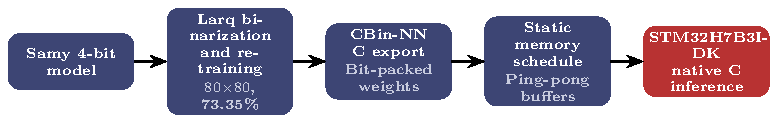
\includegraphics[width=\linewidth]{fig_cbinnn_pipeline.pdf}
  \caption{CBin-NN binary deployment pipeline for the binarized Samy model.}
  \label{fig:cbinnpipeline}
\end{figure}

% ============================================================
\section{Experimental Results}
\label{sec:results}

\begin{table}[t]
\centering
\caption{Pareto-optimal architectures (search accuracy = proxy metric on WakeVision search subset).}
\label{tab:pareto}
\begin{tabular}{@{}ccc@{}}
\toprule
\textbf{Key} & \textbf{OPs (M)} & \textbf{Search Acc.\ (\%)} \\
\midrule
3 & 3.85 & 87.39 \\
4 & 4.40 & 87.74 \\
5 & 5.24 & 87.77 \\
6 & 6.03 & 87.81 \\
\bottomrule
\end{tabular}
\end{table}

\begin{table}[t]
\centering
\caption{Accuracy vs.\ WakeVision baselines. Baselines from~\cite{banbury2025wakevision}.}
\label{tab:baselines}
\resizebox{\columnwidth}{!}{%
\begin{tabular}{@{}lccc@{}}
\toprule
\textbf{Model} & \textbf{Input} & \textbf{MACs (M)} & \textbf{Acc.\ (\%)} \\
\midrule
MCUNet-320kB~\cite{lin2020mcunet}              & $144 \times 144$ & 55.77 & \textbf{85.9} \\
MobileNetV2~0.25~\cite{sandler2018mobilenetv2} & $224 \times 224$ & 36 & 84.7 \\
MCUNet-5fps~\cite{lin2020mcunet}               & $80 \times 80$   & 12 & 83.1 \\
MCUNet-10fps~\cite{lin2020mcunet}              & $64 \times 64$   &  6 & 82.0 \\
Samy (4-bit)                 & $80 \times 80$   & \textbf{5.58}     & 79.9  \\
\midrule
NAS-BNN-Key4 (Ours)    & $128 \times 128$ & 347.66 (logical) & 80.41 \\
Binary Samy (CBin-NN) (Ours)     & $80 \times 80$   & \textbf{5.58}      & 73.35 \\
\bottomrule
\end{tabular}}
\end{table}

\begin{table*}[t]
\centering
\caption{Resource profile comparison on STM32H7B3I-DK}
\label{tab:deployment}
\resizebox{\textwidth}{!}{%
\begin{tabular}{@{}llrrrrr@{}}
\toprule
\textbf{Model} & \textbf{Input} & \textbf{Latency (ms)} & \textbf{Power (mW)} & \textbf{Energy (mJ)} & \textbf{RAM (KiB)} & \textbf{Flash (KiB)} \\
\midrule
MCUNet-320kB~\cite{lin2020mcunet}      & $144 \times 144$ & 410    & 90  & 36.9 & 393            & 924 \\
NAS-BNN Key~4 (ours) & $32 \times 32$   & 50.29 & \textbf{60} & 3.02 & 110 & 418 \\
Samy (4-bit)              & $80 \times 80$   & 37.4   & 100 & 3.7  & 26.98          & 56.62 \\
Binary Samy (CBin-NN) (ours)                            & $80 \times 80$   & \textbf{30.5}   & 80  & \textbf{2.4}  & \textbf{9.38}           & \textbf{7.03} \\
\bottomrule
\end{tabular}}
\end{table*}

The experimental evaluation focuses on the practical viability of the obtained BNN models for visual wake-word tasks on MCU-class hardware.
Since BNN efficiency depends not only on arithmetic cost but also on memory planning and operator support, WakeVision accuracy alone is insufficient to characterize the resulting models.
We therefore evaluate each candidate both as a classifier and as a deployed model, reporting test-set accuracy together with measured latency, energy, RAM, and Flash usage on the STM32H7B3I-DK.
This allows NAS-derived BNNs and WakeVision reference models to be compared under the constraints that determine actual deployment feasibility.

We used the WakeVision dataset~\cite{banbury2025wakevision} for binary person detection. The full training split contains 5{,}760{,}428 images, and the official test set contains 55{,}762 images balanced between person and no-person classes. Images are resized to $128 \times 128$ and normalized to $[-1,+1]$ per-channel. Supernet pre-training runs for 10 epochs on an NVIDIA RTX~4080 (batch 128, learning rate $2.5\times10^{-3}$, cosine annealing) on a representative WakeVision subset ($\sim${7.2}\% of the original), and fine-tuning runs for 30 epochs (batch 256, learning rate $1\times10^{-4}$) on the full 5.76\,M-image training set. The evolutionary search evaluates 250 unique architectures (population 50, 10 generations) within a 3.8--6.2\,M-OPs target range.

Table~\ref{tab:pareto} lists the four Pareto-optimal architectures found by the search defined by target M-OPs.
Despite sampling only 250 of an estimated $3.3\times10^{17}$ possible configurations, the Diversity-Aware Pareto Selection identifies a well-spread front spanning 3.85--6.03\,M-OPs.
The search-phase accuracy (proxy metric) clusters tightly at 87.39--87.81\%, confirming that the search is not over-fitting to a particular cost point; final accuracy after full-dataset fine-tuning is reported in Table~\ref{tab:baselines}.

Table~\ref{tab:baselines} compares NAS-BNN Key~4 against published WakeVision baselines from the official model zoo~\cite{banbury2025wakevision}. Key~4 achieves 80.41\% accuracy at 4.40\,M composite OPs, making it the selected candidate for MCU deployment as the best trade-off between accuracy and computational cost on the binary Pareto front.

Against the best baseline, MCUNet-320kB (85.9\% at 55.77\,M-MACs), Key~4 trades 5.5\,pp of accuracy for a binary execution path that operates on bit-packed weights and activations. The MAC count we report for Key~4 in Table~\ref{tab:baselines} is the raw logical multiply-accumulate total (347.66\,M); on hardware with native XNOR-popcount support each binary MAC costs roughly $1/32$ of a float MAC, so the wall-clock comparison is best read from the deployment results in Table~\ref{tab:deployment} rather than from the MAC tally itself. The obtained binary model, in contrast, retains the same 5.58\,M-MAC budget as the original backbone but runs every operation on the binary path, which is what makes its single-digit-kilobyte footprint and millisecond-scale latency possible.

Table~\ref{tab:deployment} reports measured deployment metrics on the STM32H7B3I-DK across four configurations: MCUNet-320kB, our Key~4 deployed via TFLM+LCE, Samy model, and our binarized model converted with CBin-NN.

MCUNet-320kB achieves 85.9\% accuracy at 410\,ms with 36.9\,mJ per inference, 924\,KiB Flash and 393\,KiB RAM.

NAS-BNN Key~4, deployed at $32 \times 32$ native input via TFLM+LCE, runs in \STMLATAVG{} with \STMARENAKIB{} peak RAM and 418\,KiB Flash; at matched input resolution ($128 \times 128$) it can alternatively be run via a 16-tile 2D streaming scheme at 799.58\,ms, enabling full-resolution binary inference within the 480\,KiB SRAM budget.

The Samy model runs in 37.4\,ms at 3.7\,mJ with 56.62\,KiB Flash and 26.98\,KiB RAM ($79.9\%$ accuracy).

The proposed binarized model, after CBin-NN deployment, achieves the best overall trade-off: 30.5\,ms latency, 80\,mW power, 2.4\,mJ energy, 7.03\,KiB Flash and 9.38\,KiB RAM at 73.35\% accuracy. This represents a $13.4\times$ latency reduction, $15.4\times$ energy reduction and $\sim$$130\times$ Flash reduction versus MCUNet-320kB at a 12.55\,pp accuracy cost.

% ============================================================
\section{Discussion}
\label{sec:discussion}

A core question this paper answers is whether NAS-BNN architectures can be deployed at all on a microcontroller. The answer is yes, but with significant engineering effort: the LCE custom operators require a tailored runtime that neither X-CUBE-AI nor standard TFLM support out of the box, and the memory footprint requires a spatial tiling scheme that is not part of any standard inference toolkit.

A subtle point worth highlighting concerns the relationship between binarization and memory footprint. The 418\,KiB Flash footprint of Key~4 is substantially larger than the 320\,KiB of MCUNet-320kB, despite the BNN performing far fewer effective operations, because Flash still has to store the model's packed binary weight buffers, and at 1\,bit per weight with 512 channels in the final stage these tensors accumulate to hundreds of kilobytes. The efficiency gain of binarization shows up in inference compute (XNOR-popcount replacing MAC), not in weight memory, relative to MCUNet-320kB, and practitioners targeting Flash-constrained deployments should account for this distinction.

The direct binarization route starts from a much smaller hardware-aware backbone. Moreover, it exploits the CBin-NN's highly-optimized bit-packing. Overall, this leads the Flash occupation to collapse to 7.03\,KiB (2+ orders of magnitude less than MCUNet-320kB), stressing that the Flash savings expected from binarization demand a compact source architecture and an optimized binarization engine.

The MAC counts reported in Table~\ref{tab:baselines} are raw logical multiply-accumulate operations and should not be read as a direct cost proxy across bit-widths. NAS-BNN-Key4 reports 347.66\,M logical MACs, which is more than six times the 55.77\,M of MCUNet-320kB, yet on hardware with native XNOR-popcount support such as LCE on the Cortex-M7 32-bit SIMD path each binary MAC costs roughly $1/32$ of a float MAC, so the wall-clock advantage emerges at runtime rather than from the MAC tally itself. On hardware without dedicated binary instructions this advantage collapses: a generic int8 \texttt{Conv2D} path would not deliver proportional speedup. The latency reported for the STM32H7B3I-DK is therefore contingent on the LCE bit-packed binary kernels~\cite{bannink2021larq} compiling to XNOR+popcount sequences, a behaviour consistent with CBin-NN~\cite{sakr2024cbinnn}: BNN runtime gains over int8 baselines disappear on hardware without dedicated binary execution units.

The 12.55\,pp accuracy gap between the proposed binary model (73.35\%) and MCUNet-320kB (85.9\%) is the direct cost of strict 1-bit quantization throughout the network. For always-on person sensing where inference must run continuously on a battery-powered device, the $13.4\times$ latency reduction and $15.4\times$ energy reduction of the binary path may well be preferable to the higher accuracy but $>$400\,ms latency of MCUNet-320kB; the appropriate choice depends on the application's false-negative tolerance.

Some limitations remain. The accuracy gap to MCUNet-320kB is unlikely to close with additional fine-tuning epochs alone, and partial bit-width relaxation in the early stem or distillation from a stronger teacher would likely be needed. The 2D spatial tiling scheme requires that the backbone's spatial stride pattern evenly divides both tile dimensions, so architectures with odd strides or cross-tile padding dependencies would need a modified streaming strategy with overlap regions. Finally, per-key STM32 latency curves for Keys 3, 5, and 6 are left to future work.

% ============================================================
\section{Conclusions}
\label{sec:conclusion}

We have demonstrated extreme binary quantization for visual wake-up of conversational agents on an industry-grade high-performance microcontroller (STM32H7B3I-DK, Cortex-M7, 280\,MHz, 480\,KiB internal SRAM).
Two complementary deployments are reported.
On the NAS-BNN side, we built a complete pipeline from binary supernet search through Larq Compute Engine TFLite export to a custom Cortex-M7 firmware, and showed that a 16-tile 2D spatial input-streaming scheme keeps full-resolution Key~4 inference within the SRAM budget at 80.41\% accuracy and 799.58\,ms.
On the model-centric side, we binarized the official Wakevision 4-bit Samy model and converted it to C with the CBin-NN inference engine, achieving the best overall efficiency trade-off, latency (30.5\,ms), power (80\,mW), energy (2.4\,mJ), Flash (7.03\,KiB) and RAM (9.38\,KiB) at acceptable accuracy cost (73.35\%) on the same board.

Three concrete takeaways follow.
(i)~NAS-BNN architectures are deployable on Cortex-M hardware, but require a custom binary-kernel runtime and spatial memory tiling to meet realistic SRAM budgets.
(ii)~A hardware-aware reference architecture combined with a dedicated binary inference engine (CBin-NN) largely outperforms an MCU-unaware NAS pipeline across every measured deployment metric, motivating the integration of binary-kernel constraints directly into the NAS objective.
(iii)~Binarization with (cross-channel) bit-packed weights collapses Flash by more than two orders of magnitude versus int8 references, while ping-pong activation buffering reduces RAM to single-digit kilobytes, making always-on visual wake-up feasible within minimal-footprint hardware budgets.

The findings of this study identify key directions for future research, such as: (i) binary-aware training with the BOP optimizer~\cite{bannink2021larq} to address the accuracy gap, (ii) integration of binary-kernel constraints directly into the NAS optimization objective, (iii) stride-aware tile overlap to generalize the streaming scheme, and (iv) extension to multi-class detection and keyword spotting on MLPerf Tiny~\cite{banbury2021mlperftiny} benchmarks.

% ============================================================
\balance
\bibliographystyle{IEEEtran}
\bibliography{references}

\end{document}
